\documentclass{beamer}
\usepackage{../../shared/styles/custom}
\usepackage{../../shared/styles/conventions}

\usepackage{grffile}
\usepackage{tikz}
\usetikzlibrary{matrix,positioning,backgrounds,fit,calc,arrows.meta,shapes}

\title{Matrix Factorization for Movie Recommendation Systems}
\date{\today}
\author{Nipun Batra}
\institute{IIT Gandhinagar}

\begin{document}
\maketitle

\begin{frame}{Today's Learning Journey}
\begin{itemize}[<+->]
    \item \textbf{The Problem}: Why do we need recommendation systems?
    \item \textbf{Matrix View}: How ratings become a mathematical problem
    \item \textbf{Key Insight}: Matrix factorization as the solution
    \item \textbf{Step-by-Step}: Building intuition with examples
    \item \textbf{Algorithms}: ALS vs Gradient Descent
    \item \textbf{Practice}: Hands-on understanding
\end{itemize}
\end{frame}

\section{Problem Setup}

\begin{frame}{The Movie Recommendation Challenge}
\begin{columns}[T]
\begin{column}{0.5\textwidth}
\textbf{Real-World Scenario:}
\begin{itemize}[<+->]
    \item Netflix: 200M+ users, 15K+ titles
    \item Amazon: 300M+ users, millions of products  
    \item Spotify: 400M+ users, 70M+ songs
    \item Most ratings are missing!
\end{itemize}

\pause
\textbf{Think About It:}
\begin{itemize}[<+->]
    \item You've rated ~100 movies out of 15,000
    \item Your friend has similar but different tastes
    \item How do we predict what you'll like?
\end{itemize}
\end{column}
\begin{column}{0.5\textwidth}
\only<4->{
\begin{center}
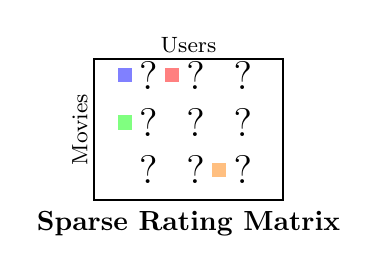
\begin{tikzpicture}[scale=0.6]
    \draw[thick] (0,0) rectangle (4,3);
    \node at (2,3.3) {\footnotesize Users};
    \node[rotate=90] at (-0.3,1.5) {\footnotesize Movies};
    
    % Some filled squares (known ratings)
    \fill[blue!50] (0.5,2.5) rectangle (0.8,2.8);
    \fill[red!50] (1.5,2.5) rectangle (1.8,2.8);
    \fill[green!50] (0.5,1.5) rectangle (0.8,1.8);
    \fill[orange!50] (2.5,0.5) rectangle (2.8,0.8);
    
    % Question marks for missing
    \node at (1.15,2.65) {\Large ?};
    \node at (2.15,2.65) {\Large ?};
    \node at (3.15,2.65) {\Large ?};
    \node at (1.15,1.65) {\Large ?};
    \node at (2.15,1.65) {\Large ?};
    \node at (3.15,1.65) {\Large ?};
    \node at (1.15,0.65) {\Large ?};
    \node at (2.15,0.65) {\Large ?};
    \node at (3.15,0.65) {\Large ?};
    
    \node at (2,-0.5) {\textbf{Sparse Rating Matrix}};
\end{tikzpicture}
\end{center}
}
\end{column}
\end{columns}
\end{frame}

\begin{frame}{Pop Quiz 1: Understanding the Scale}
\begin{tcolorbox}[colback=blue!5!white,colframe=blue!75!black,title=Quick Question]
If Netflix has 200 million users and 15,000 movies, how many possible ratings exist?

\pause
\vspace{0.5cm}
\textbf{Answer:} $200 \times 10^6 \times 15 \times 10^3 = 3 \times 10^{12}$ possible ratings!

\pause
But typical users rate only 20-100 movies. What percentage of the matrix is filled?

\pause
\textbf{Answer:} $\frac{100}{15000} = 0.67\%$ - extremely sparse!
\end{tcolorbox}
\end{frame}

\begin{frame}{Mathematical Problem Setup}
\textbf{The Rating Matrix} $\mA \in \Real^{N \times M}$:
\pause

\begin{equation*}
\mA = \begin{bmatrix}
a_{11} & ? & a_{13} & ? & \cdots \\
? & a_{22} & ? & a_{24} & \cdots \\
a_{31} & ? & ? & a_{34} & \cdots \\
\vdots & \vdots & \vdots & \vdots & \ddots
\end{bmatrix}
\end{equation*}

\pause
\begin{itemize}[<+->]
    \item \textbf{Rows}: Users $u_1, u_2, \ldots, u_N$ 
    \item \textbf{Columns}: Movies $m_1, m_2, \ldots, m_M$
    \item \textbf{Entries}: $a_{ij} \in \{1,2,3,4,5\}$ (when observed)
    \item \textbf{Challenge}: Predict missing entries $?$
    \item \textbf{Notation}: $\Omega = \{(i,j) : a_{ij} \text{ is observed}\}$
\end{itemize}
\end{frame}

\begin{frame}{Concrete Example: Our Movie Dataset}
Let's work with a small, concrete example:

\pause
\begin{center}
\renewcommand{\arraystretch}{1.2}
\begin{tabular}{l|ccccc}
\toprule
\textbf{User} & \textbf{Sholay} & \textbf{Swades} & \textbf{Batman} & \textbf{Interstellar} & \textbf{Shawshank} \\
\midrule
Alice & \textcolor{blue}{5} & \textcolor{blue}{4} & \textcolor{red}{2} & \textcolor{red}{3} & \textcolor{red}{2} \\
Bob & \textcolor{red}{?} & \textcolor{blue}{5} & \textcolor{red}{1} & \textcolor{blue}{4} & \textcolor{red}{?} \\
Carol & \textcolor{blue}{4} & \textcolor{red}{?} & \textcolor{red}{1} & \textcolor{blue}{5} & \textcolor{red}{?} \\
\bottomrule
\end{tabular}
\end{center}

\pause
\textbf{Observations:}
\begin{itemize}[<+->]
    \item Alice loves Bollywood films (Sholay, Swades)
    \item Carol enjoys Sci-Fi (Interstellar)  
    \item Can we predict Bob's rating for Sholay?
    \item Can we predict Carol's rating for Swades?
\end{itemize}
\end{frame}

\section{Key Insight: Latent Features}

\begin{frame}{Before We Dive In: A Simple Question}
\begin{center}
\Large \textbf{Why do you like the movies you like?}
\end{center}

\pause
\begin{columns}[T]
\begin{column}{0.5\textwidth}
\textbf{Maybe because of:}
\begin{itemize}[<+->]
    \item Genre (Action, Romance, Comedy)
    \item Star cast (Shah Rukh Khan, Tom Cruise)
    \item Director (Christopher Nolan, Rajkumar Hirani)
    \item Language (Hindi, English, Tamil)
    \item Era (90s classics, modern CGI)
\end{itemize}
\end{column}
\begin{column}{0.5\textwidth}
\only<6->{
\textbf{Key Insight:}
\begin{itemize}
    \item Your taste = combination of preferences
    \item Movie appeal = combination of features
    \item \textcolor{red}{But we don't know these explicitly!}
\end{itemize}
}
\end{column}
\end{columns}
\end{frame}

\begin{frame}{The Core Insight: Hidden Patterns}
\begin{columns}[T]
\begin{column}{0.6\textwidth}
\textbf{Hypothesis:} User preferences and movie characteristics can be captured by a small number of \textbf{latent features}.

\pause
\textbf{Intuition:} Think of latent features as ``hidden DNA'' of movies and users!

\pause
\vspace{0.5cm}
\textbf{For Movies:}
\begin{itemize}[<+->]
    \item Bollywood vs Hollywood
    \item Action vs Drama  
    \item Comedy vs Serious
    \item Runtime (Short vs Long)
    \item Year (Classic vs Modern)
\end{itemize}
\end{column}
\begin{column}{0.4\textwidth}
\only<6->{
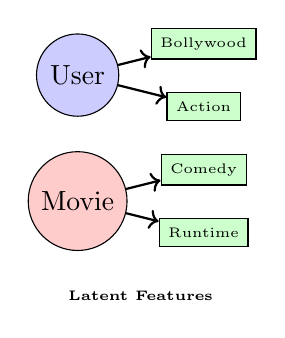
\begin{tikzpicture}[scale=0.8]
    \node[draw, circle, fill=blue!20] (user) at (0,2) {User};
    \node[draw, circle, fill=red!20] (movie) at (0,0) {Movie};
    
    \node[draw, rectangle, fill=green!20] (f1) at (2,2.5) {\tiny Bollywood};
    \node[draw, rectangle, fill=green!20] (f2) at (2,1.5) {\tiny Action};
    \node[draw, rectangle, fill=green!20] (f3) at (2,0.5) {\tiny Comedy};
    \node[draw, rectangle, fill=green!20] (f4) at (2,-0.5) {\tiny Runtime};
    
    \draw[->, thick] (user) -- (f1);
    \draw[->, thick] (user) -- (f2);
    \draw[->, thick] (movie) -- (f3);
    \draw[->, thick] (movie) -- (f4);
    
    \node at (1,-1.5) {\tiny \textbf{Latent Features}};
\end{tikzpicture}
}
\end{column}
\end{columns}
\end{frame}

\begin{frame}{Step 1: Define Movie Features Explicitly}
Let's manually define features for our 5 movies:

\pause
\begin{center}
\renewcommand{\arraystretch}{1.3}
\begin{tabular}{l|ccc}
\toprule
\textbf{Movie} & \textbf{Bollywood} & \textbf{Sci-Fi} & \textbf{Drama} \\
\midrule
Sholay & \textcolor{blue}{0.95} & \textcolor{red}{0.10} & \textcolor{orange}{0.85} \\
Swades & \textcolor{blue}{1.00} & \textcolor{red}{0.20} & \textcolor{orange}{0.90} \\
Batman & \textcolor{blue}{0.05} & \textcolor{red}{0.80} & \textcolor{orange}{0.30} \\
Interstellar & \textcolor{blue}{0.05} & \textcolor{red}{0.95} & \textcolor{orange}{0.70} \\
Shawshank & \textcolor{blue}{0.05} & \textcolor{red}{0.15} & \textcolor{orange}{0.95} \\
\bottomrule
\end{tabular}
\end{center}

\pause
\textbf{Movie Feature Matrix} $\mH \in \Real^{3 \times 5}$:
\begin{equation*}
\mH = \begin{bmatrix}
\textcolor{blue}{0.95} & \textcolor{blue}{1.00} & \textcolor{blue}{0.05} & \textcolor{blue}{0.05} & \textcolor{blue}{0.05} \\
\textcolor{red}{0.10} & \textcolor{red}{0.20} & \textcolor{red}{0.80} & \textcolor{red}{0.95} & \textcolor{red}{0.15} \\
\textcolor{orange}{0.85} & \textcolor{orange}{0.90} & \textcolor{orange}{0.30} & \textcolor{orange}{0.70} & \textcolor{orange}{0.95}
\end{bmatrix}
\end{equation*}
\end{frame}

\begin{frame}{Step 2: What About User Preferences?}
\textbf{User Feature Matrix} $\mW \in \Real^{3 \times 3}$ represents user preferences:

\pause
\begin{equation*}
\mW = \begin{bmatrix}
w_{11} & w_{12} & w_{13} \\
w_{21} & w_{22} & w_{23} \\
w_{31} & w_{32} & w_{33}
\end{bmatrix}
\end{equation*}

\pause
Where row $i$ represents user $i$'s affinity for:
\begin{itemize}[<+->]
    \item $w_{i1}$: Bollywood preference
    \item $w_{i2}$: Sci-Fi preference  
    \item $w_{i3}$: Drama preference
\end{itemize}

\pause
\textbf{Key Question:} How do we learn these $w_{ij}$ values from observed ratings?
\end{frame}

\begin{frame}{Step 3: The Matrix Factorization Idea}
\textbf{Core Hypothesis:} Rating = User preferences · Movie features

\pause
\begin{equation*}
\boxed{a_{ij} \approx \vw_i^T \vh_j = \sum_{k=1}^r w_{ik} h_{kj}}
\end{equation*}

\pause
\textbf{In Matrix Form:}
\begin{equation*}
\boxed{\mA \approx \mW \mH}
\end{equation*}

\pause
\begin{center}
$\mA_{3 \times 5} =
\begin{bmatrix}
5 & 4 & 2 & 3 & 2 \\
? & 5 & 1 & 4 & ? \\
4 & ? & 1 & 5 & ? 
\end{bmatrix}
\approx
\begin{bmatrix}
w_{11} & w_{12} & w_{13} \\
w_{21} & w_{22} & w_{23} \\
w_{31} & w_{32} & w_{33}
\end{bmatrix}
\begin{bmatrix}
0.95 & 1.00 & 0.05 & 0.05 & 0.05 \\
0.10 & 0.20 & 0.80 & 0.95 & 0.15 \\
0.85 & 0.90 & 0.30 & 0.70 & 0.95
\end{bmatrix}
= \mW_{3 \times 3} \mH_{3 \times 5}$
\end{center}
\end{frame}

\begin{frame}{Step 4: Understanding the Calculation}
\textbf{Let's think step by step...}

\pause
\begin{columns}[T]
\begin{column}{0.5\textwidth}
\textbf{Alice's Profile:}
\begin{itemize}[<+->]
    \item How much does she like Bollywood? $w_{11}$
    \item How much does she like Action? $w_{12}$
    \item How much does she like Comedy? $w_{13}$
\end{itemize}
\end{column}
\begin{column}{0.5\textwidth}
\only<4->{
\textbf{Sholay's DNA:}
\begin{itemize}
    \item Bollywood-ness: 0.95 (very high!)
    \item Action-ness: 0.10 (low)
    \item Comedy-ness: 0.85 (high)
\end{itemize}
}
\end{column}
\end{columns}

\pause
\vspace{0.5cm}
\textbf{The Magic Formula:} 
$$\text{Alice's rating} = \text{Alice's preferences} \cdot \text{Sholay's features}$$
\end{frame}

\begin{frame}{Step 4: Detailed Calculation Example}
Let's compute Alice's predicted rating for Sholay:

\pause
\textbf{Alice's preferences:} $\vw_1 = [w_{11}, w_{12}, w_{13}]$
\textbf{Sholay's features:} $\vh_1 = [0.95, 0.10, 0.85]^T$

\pause
\begin{align}
\hat{a}_{11} &= \vw_1^T \vh_1 \\
&= w_{11} \cdot 0.95 + w_{12} \cdot 0.10 + w_{13} \cdot 0.85
\end{align}

\pause
\textbf{Goal:} Find $w_{11}, w_{12}, w_{13}$ such that $\hat{a}_{11} \approx 5$ (Alice's actual rating)
\end{frame}

\begin{frame}{Pop Quiz 2: Matrix Dimensions}
\begin{tcolorbox}[colback=green!5!white,colframe=green!75!black,title=Dimension Check]
If we have $N$ users, $M$ movies, and $r$ latent features:

\pause
\begin{enumerate}[<+->]
    \item What are the dimensions of $\mA$? 
    \item What are the dimensions of $\mW$?
    \item What are the dimensions of $\mH$?
    \item How many parameters do we need to learn?
\end{enumerate}

\pause
\textbf{Answers:}
\begin{enumerate}
    \item $\mA \in \Real^{N \times M}$
    \item $\mW \in \Real^{N \times r}$ 
    \item $\mH \in \Real^{r \times M}$
    \item Total parameters: $Nr + rM = r(N + M)$
\end{enumerate}

\pause
\textbf{Key Insight:} If $r \ll \min(N,M)$, we have huge parameter reduction!
\end{tcolorbox}
\end{frame}

\section{Learning the Factorization}

\begin{frame}{The Optimization Problem}
\textbf{Objective:} Minimize prediction error on observed ratings only

\pause
\begin{equation*}
\boxed{\minimize_{\mW,\mH} \sum_{(i,j) \in \Omega} (a_{ij} - \vw_i^T \vh_j)^2}
\end{equation*}

\pause
\textbf{In Matrix Notation:}
\begin{equation*}
\boxed{\minimize_{\mW,\mH} \|P_\Omega(\mA - \mW\mH)\|_F^2}
\end{equation*}

\pause
Where:
\begin{itemize}[<+->]
    \item $P_\Omega(\cdot)$: projection onto observed entries
    \item $\|\cdot\|_F$: Frobenius norm
    \item $\Omega$: set of observed $(i,j)$ pairs
\end{itemize}
\end{frame}

\begin{frame}{Why This is Challenging}
\textbf{Problem Characteristics:}
\begin{itemize}[<+->]
    \item \textbf{Non-convex:} Multiple local minima exist
    \item \textbf{Bilinear:} Linear in $\mW$ when $\mH$ fixed, and vice versa
    \item \textbf{Large-scale:} Millions of users and items
    \item \textbf{Sparse:} Only 0.1-1\% of entries observed
\end{itemize}

\pause
\textbf{Key Insight:} While non-convex jointly, it's convex in each matrix individually!
\end{frame}

\section{Algorithm 1: Alternating Least Squares (ALS)}

\begin{frame}{ALS: The Big Picture}
\textbf{Alternating Least Squares Strategy:}

\pause
\begin{enumerate}[<+->]
    \item \textbf{Initialize:} $\mW^{(0)}$ and $\mH^{(0)}$ randomly
    \item \textbf{Repeat until convergence:}
    \begin{enumerate}
        \item \textbf{Fix $\mH$, solve for $\mW$:} Each row independently
        \item \textbf{Fix $\mW$, solve for $\mH$:} Each column independently  
    \end{enumerate}
    \item Each subproblem is a standard least squares problem!
\end{enumerate}

\pause
\begin{center}
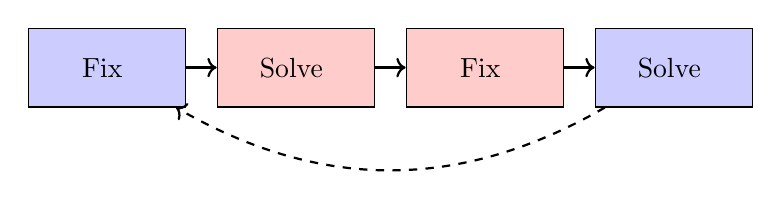
\begin{tikzpicture}[scale=0.8]
    \node[draw, fill=blue!20, minimum width=2cm, minimum height=1cm] (W) at (0,0) {Fix $\mW$};
    \node[draw, fill=red!20, minimum width=2cm, minimum height=1cm] (H) at (3,0) {Solve $\mH$};
    \node[draw, fill=red!20, minimum width=2cm, minimum height=1cm] (W2) at (6,0) {Fix $\mH$};
    \node[draw, fill=blue!20, minimum width=2cm, minimum height=1cm] (H2) at (9,0) {Solve $\mW$};
    
    \draw[->, thick] (W) -- (H);
    \draw[->, thick] (H) -- (W2);
    \draw[->, thick] (W2) -- (H2);
    \draw[->, thick, dashed] (H2) to[bend left] (W);
\end{tikzpicture}
\end{center}
\end{frame}

\begin{frame}{ALS Step 1: Updating User Features}
\textbf{Fix $\mH$, solve for each user $i$ independently:}

\pause
\begin{equation*}
\minimize_{\vw_i} \sum_{j: (i,j) \in \Omega} (a_{ij} - \vw_i^T \vh_j)^2
\end{equation*}

\pause
\textbf{Matrix Form for User $i$:}
Let $\Omega_i = \{j: (i,j) \in \Omega\}$ (movies rated by user $i$)

\pause
\begin{align}
\vy_i &= [a_{i,j_1}, a_{i,j_2}, \ldots, a_{i,j_{|\Omega_i|}}]^T \\
\mX_i &= [\vh_{j_1}, \vh_{j_2}, \ldots, \vh_{j_{|\Omega_i|}}]^T
\end{align}

\pause
\textbf{Least Squares Solution:}
\begin{equation*}
\boxed{\vw_i^* = (\mX_i^T \mX_i)^{-1} \mX_i^T \vy_i}
\end{equation*}
\end{frame}

\begin{frame}{ALS Step 1: Concrete Example}
\textbf{Update Alice's preferences ($\vw_1$):}

Alice rated: Sholay(5), Swades(4), Batman(2), Interstellar(3), Shawshank(2)

\pause
\begin{align}
\vy_1 &= \begin{bmatrix} 5 \\ 4 \\ 2 \\ 3 \\ 2 \end{bmatrix} \\
\mX_1 &= \begin{bmatrix} 
0.95 & 0.10 & 0.85 \\
1.00 & 0.20 & 0.90 \\
0.05 & 0.80 & 0.30 \\
0.05 & 0.95 & 0.70 \\
0.05 & 0.15 & 0.95
\end{bmatrix}
\end{align}

\pause
\textbf{Solution:} $\vw_1^* = (\mX_1^T \mX_1)^{-1} \mX_1^T \vy_1$

This gives us Alice's feature preferences!
\end{frame}

\begin{frame}{ALS Step 2: Updating Movie Features}
\textbf{Fix $\mW$, solve for each movie $j$ independently:}

\pause
\begin{equation*}
\minimize_{\vh_j} \sum_{i: (i,j) \in \Omega} (a_{ij} - \vw_i^T \vh_j)^2
\end{equation*}

\pause
\textbf{Matrix Form for Movie $j$:}
Let $\Omega_j = \{i: (i,j) \in \Omega\}$ (users who rated movie $j$)

\pause
\begin{align}
\vy_j &= [a_{i_1,j}, a_{i_2,j}, \ldots, a_{i_{|\Omega_j|},j}]^T \\
\mX_j &= [\vw_{i_1}, \vw_{i_2}, \ldots, \vw_{i_{|\Omega_j|}}]^T
\end{align}

\pause
\textbf{Least Squares Solution:}
\begin{equation*}
\boxed{\vh_j^* = (\mX_j^T \mX_j)^{-1} \mX_j^T \vy_j}
\end{equation*}
\end{frame}

\begin{frame}{ALS: Complete Algorithm}
\begin{algorithm}[H]
\textbf{Input:} Rating matrix $\mA$, rank $r$, max iterations $T$
\begin{enumerate}[<+->]
    \item \textbf{Initialize:} $\mW^{(0)} \in \Real^{N \times r}$, $\mH^{(0)} \in \Real^{r \times M}$ randomly
    \item \textbf{For} $t = 1, 2, \ldots, T$:
    \begin{enumerate}
        \item \textbf{Update Users:} For each user $i = 1, \ldots, N$:
        $$\vw_i^{(t)} = (\mX_i^T \mX_i)^{-1} \mX_i^T \vy_i$$
        \item \textbf{Update Movies:} For each movie $j = 1, \ldots, M$:
        $$\vh_j^{(t)} = (\mX_j^T \mX_j)^{-1} \mX_j^T \vy_j$$
    \end{enumerate}
    \item \textbf{Check Convergence:} Stop if $\|\mW^{(t)}\mH^{(t)} - \mW^{(t-1)}\mH^{(t-1)}\|_F < \epsilon$
\end{enumerate}
\textbf{Output:} $\mW^{(T)}$, $\mH^{(T)}$
\end{algorithm}
\end{frame}

\section{Algorithm 2: Gradient Descent}

\begin{frame}{Gradient Descent Approach}
\textbf{Simultaneous Updates:} Update both $\mW$ and $\mH$ together

\pause
\textbf{Objective Function:}
\begin{equation*}
L(\mW, \mH) = \sum_{(i,j) \in \Omega} (a_{ij} - \vw_i^T \vh_j)^2
\end{equation*}

\pause
\textbf{Gradients:}
\begin{align}
\frac{\partial L}{\partial \vw_i} &= -2 \sum_{j: (i,j) \in \Omega} (a_{ij} - \vw_i^T \vh_j) \vh_j \\
\frac{\partial L}{\partial \vh_j} &= -2 \sum_{i: (i,j) \in \Omega} (a_{ij} - \vw_i^T \vh_j) \vw_i
\end{align}
\end{frame}

\begin{frame}{SGD: Learning Like a Human}
\begin{center}
\textbf{Imagine you're learning someone's taste in movies...}
\end{center}

\pause
\begin{columns}[T]
\begin{column}{0.5\textwidth}
\textbf{Your Process:}
\begin{enumerate}[<+->]
    \item Make a guess about their rating
    \item See their actual rating
    \item Adjust your understanding
    \item Repeat for next movie
\end{enumerate}
\end{column}
\begin{column}{0.5\textwidth}
\only<5->{
\textbf{SGD does exactly this!}
\begin{itemize}
    \item One rating at a time
    \item Small adjustments
    \item Gradually improves
\end{itemize}
}
\end{column}
\end{columns}
\end{frame}

\begin{frame}{Stochastic Gradient Descent (SGD)}
\textbf{For each observed rating $(i,j) \in \Omega$:}

\pause
\begin{enumerate}[<+->]
    \item \textbf{Predict:} $\hat{a}_{ij} = \vw_i^T \vh_j$
    \item \textbf{Compute Error:} $e_{ij} = a_{ij} - \hat{a}_{ij}$  
    \item \textbf{Update:}
    \begin{align}
    \vw_i &\leftarrow \vw_i + \alpha \cdot e_{ij} \cdot \vh_j \\
    \vh_j &\leftarrow \vh_j + \alpha \cdot e_{ij} \cdot \vw_i
    \end{align}
\end{enumerate}

\pause
\textbf{Intuition:}
\begin{itemize}[<+->]
    \item If $e_{ij} > 0$: Predicted rating too low → Increase similarity
    \item If $e_{ij} < 0$: Predicted rating too high → Decrease similarity
    \item Learning rate $\alpha$ controls step size
\end{itemize}
\end{frame}

\begin{frame}{SGD: Step-by-Step Example}
\textbf{Example:} Alice rates Sholay as 5, but we predict 3.2

\pause
\begin{align}
\text{Current: } &\vw_1 = [0.4, 0.2, 0.3], \quad \vh_1 = [0.95, 0.10, 0.85] \\
\text{Prediction: } &\hat{a}_{11} = 0.4 \times 0.95 + 0.2 \times 0.10 + 0.3 \times 0.85 = 0.655 \\
\text{Error: } &e_{11} = 5 - 0.655 = 4.345
\end{align}

\pause
\textbf{Updates with $\alpha = 0.01$:}
\begin{align}
\vw_1 &\leftarrow [0.4, 0.2, 0.3] + 0.01 \times 4.345 \times [0.95, 0.10, 0.85] \\
&= [0.4413, 0.2043, 0.3369] \\
\vh_1 &\leftarrow [0.95, 0.10, 0.85] + 0.01 \times 4.345 \times [0.4, 0.2, 0.3] \\
&= [0.9674, 0.1087, 0.8631]
\end{align}
\end{frame}

\begin{frame}{Pop Quiz 3: SGD Understanding}
\begin{tcolorbox}[colback=orange!5!white,colframe=orange!75!black,title=Quick Check]
A user gives a rating of 2 to a movie, but our model predicts 4.5.

\pause
\begin{enumerate}[<+->]
    \item What is the error $e_{ij}$?
    \item Should we increase or decrease the user-movie similarity?
    \item If $\alpha = 0.1$, $\vw_i = [0.8, 0.3]$, $\vh_j = [0.6, 0.9]$, what are the updates?
\end{enumerate}

\pause
\textbf{Answers:}
\begin{enumerate}
    \item $e_{ij} = 2 - 4.5 = -2.5$
    \item Decrease similarity (negative error)
    \item $\vw_i \leftarrow [0.8, 0.3] + 0.1 \times (-2.5) \times [0.6, 0.9] = [0.65, 0.075]$
    \item $\vh_j \leftarrow [0.6, 0.9] + 0.1 \times (-2.5) \times [0.8, 0.3] = [0.4, 0.825]$
\end{enumerate}
\end{tcolorbox}
\end{frame}

\section{Algorithm Comparison and Practical Considerations}

\begin{frame}{ALS vs SGD: Head-to-Head Comparison}
\begin{center}
\renewcommand{\arraystretch}{1.4}
\begin{tabular}{l|cc}
\toprule
\textbf{Aspect} & \textbf{ALS} & \textbf{SGD} \\
\midrule
\textbf{Updates} & Alternating & Simultaneous \\
\textbf{Convergence} & Faster, more stable & Slower, can oscillate \\
\textbf{Parallelization} & Excellent & Limited \\
\textbf{Memory} & Higher & Lower \\
\textbf{Implementation} & Complex & Simple \\
\textbf{Hyperparameters} & Few (rank $r$) & Many ($\alpha$, schedule) \\
\textbf{Scalability} & Very good & Good \\
\bottomrule
\end{tabular}
\end{center}

\pause
\textbf{When to Use Which?}
\begin{itemize}[<+->]
    \item \textbf{ALS:} Large-scale, production systems (Spark, distributed)
    \item \textbf{SGD:} Online learning, real-time updates, research
\end{itemize}
\end{frame}

\begin{frame}{Advanced Practical Considerations}
\textbf{Regularization:} Prevent overfitting
\begin{equation*}
\minimize_{\mW,\mH} \sum_{(i,j) \in \Omega} (a_{ij} - \vw_i^T \vh_j)^2 + \lambda(\|\mW\|_F^2 + \|\mH\|_F^2)
\end{equation*}

\pause
\textbf{Bias Terms:} Account for global, user, and item biases
\begin{equation*}
\hat{a}_{ij} = \mu + b_i + b_j + \vw_i^T \vh_j
\end{equation*}

\pause
\textbf{Implicit Feedback:} Binary observations (clicks, views)
\begin{equation*}
\text{Confidence: } c_{ij} = 1 + \alpha \cdot \text{frequency}_{ij}
\end{equation*}

\pause
\textbf{Cold Start Problem:} New users/items with no ratings
\begin{itemize}[<+->]
    \item Content-based features
    \item Demographic information  
    \item Hybrid approaches
\end{itemize}
\end{frame}

\section{Hands-On Understanding}

\begin{frame}{Let's Build Intuition: Small Example}
\textbf{Our 3×3 rating matrix:}
\begin{equation*}
\mA = \begin{bmatrix}
5 & ? & 2 \\
4 & 4 & ? \\
? & 5 & 1
\end{bmatrix}
\end{equation*}

\pause
\textbf{Goal:} Find $\mW \in \Real^{3 \times 2}$ and $\mH \in \Real^{2 \times 3}$ such that:
\begin{equation*}
\mA \approx \mW \mH = \begin{bmatrix}
w_{11} & w_{12} \\
w_{21} & w_{22} \\
w_{31} & w_{32}
\end{bmatrix}
\begin{bmatrix}
h_{11} & h_{12} & h_{13} \\
h_{21} & h_{22} & h_{23}
\end{bmatrix}
\end{equation*}

\pause
\textbf{Constraint:} Only minimize error on observed entries!
\end{frame}

\begin{frame}{Step-by-Step ALS Solution}
\textbf{Iteration 1:} Initialize randomly
\begin{equation*}
\mW^{(0)} = \begin{bmatrix} 0.5 & 0.3 \\ 0.4 & 0.6 \\ 0.2 & 0.8 \end{bmatrix}, \quad
\mH^{(0)} = \begin{bmatrix} 1.0 & 0.5 & 0.2 \\ 0.3 & 1.2 & 0.8 \end{bmatrix}
\end{equation*}

\pause
\textbf{Update User 1:} Only use observed ratings (positions 1,3)
\begin{align}
\vy_1 &= [5, 2]^T \\
\mX_1 &= \begin{bmatrix} 1.0 & 0.3 \\ 0.2 & 0.8 \end{bmatrix} \text{ (columns 1,3 of } \mH^{(0)T}\text{)}
\end{align}

\pause
\textbf{Solve:} $\vw_1^{(1)} = (\mX_1^T \mX_1)^{-1} \mX_1^T \vy_1$

Continue for all users and movies...
\end{frame}

\begin{frame}{Pop Quiz 4: Final Challenge}
\begin{tcolorbox}[colback=purple!5!white,colframe=purple!75!black,title=Master Check]
You're Netflix's lead ML engineer. You have:
\begin{itemize}
    \item 200M users, 15K movies  
    \item 20B ratings (0.67\% filled)
    \item Need real-time recommendations
    \item New users/movies arrive daily
\end{itemize}

\pause
Design your recommendation system:
\begin{enumerate}[<+->]
    \item Which algorithm: ALS or SGD? Why?
    \item What rank $r$ would you choose?
    \item How to handle new users?
    \item How to handle the scale?
\end{enumerate}

\pause
\textbf{Suggested Solution:}
\begin{itemize}
    \item \textbf{ALS} for batch processing (Spark), \textbf{SGD} for online updates
    \item $r = 50-200$ (balance between expressiveness and efficiency)
    \item Hybrid: Content-based for cold start + collaborative filtering
    \item Distributed computing, approximate algorithms, caching
\end{itemize}
\end{tcolorbox}
\end{frame}

\section{Summary and Key Takeaways}

\begin{frame}{Key Insights Summary}
\begin{enumerate}[<+->]
    \item \textbf{Sparsity $\Rightarrow$ Factorization}: Sparse rating matrices can be approximated by low-rank factorizations
    
    \item \textbf{Latent Features}: Users and items are characterized by latent factors (not manually defined!)
    
    \item \textbf{Bilinear Problem}: Non-convex jointly, but convex individually → Alternating optimization works well
    
    \item \textbf{Scale Matters}: Algorithm choice depends on data size and computational constraints
    
    \item \textbf{Real-World Complexity}: Regularization, bias terms, cold start, implicit feedback all matter
\end{enumerate}

\pause
\textbf{The Mathematical Beauty:}
\begin{equation*}
\boxed{\text{Collaborative Filtering} = \text{Matrix Factorization} = \text{Dimensionality Reduction}}
\end{equation*}
\end{frame}

\begin{frame}{Extensions and Advanced Topics}
\textbf{Beyond Basic Matrix Factorization:}

\pause
\begin{itemize}[<+->]
    \item \textbf{Non-negative Matrix Factorization (NMF)}: Interpretable factors
    
    \item \textbf{Deep Matrix Factorization}: Neural networks for non-linear patterns
    
    \item \textbf{Factorization Machines}: Handle multi-way interactions
    
    \item \textbf{Variational Autoencoders}: Probabilistic approach to recommendations
    
    \item \textbf{Graph Neural Networks}: Leverage user-item interaction graphs
    
    \item \textbf{Multi-armed Bandits}: Exploration vs exploitation in recommendations
\end{itemize}

\pause
\textbf{Applications Beyond Movies:}
\begin{itemize}[<+->]
    \item E-commerce (Amazon, eBay)
    \item Music streaming (Spotify, Apple Music)  
    \item Social media (Facebook, LinkedIn)
    \item Online advertising (Google, Facebook)
\end{itemize}
\end{frame}

\begin{frame}{Final Pop Quiz: Comprehensive Understanding}
\begin{tcolorbox}[colback=blue!5!white,colframe=blue!75!black,title=Mastery Test]
\textbf{True or False? Explain your reasoning:}

\pause
\begin{enumerate}[<+->]
    \item Matrix factorization can only work with explicit ratings
    \item ALS always converges to the global optimum  
    \item A rank-1 factorization means all users have identical preferences
    \item Adding regularization always improves recommendations
    \item SGD is better than ALS for all applications
\end{enumerate}

\pause
\textbf{Answers:}
\begin{enumerate}
    \item \textbf{False} - Works with implicit feedback too (clicks, views)
    \item \textbf{False} - Converges to local optimum (problem is non-convex)
    \item \textbf{False} - Rank-1 means one dominant pattern, not identical preferences
    \item \textbf{False} - Too much regularization can cause underfitting
    \item \textbf{False} - Choice depends on scale, parallelization needs, stability requirements
\end{enumerate}
\end{tcolorbox}
\end{frame}

\begin{frame}[standout]
\Huge \textbf{Questions?}
\vspace{1em}

\Large Thank you for your attention!
\vspace{1em}

\normalsize
Next: Deep learning approaches to recommendation systems
\end{frame}

\end{document}